% Chapter 1

\chapter{Introduction} % Write in your own chapter title
\label{Chapter1}
\lhead{Chapter 1. \emph{Introduction}} % Write in your own chapter title to set the page header


\section{The cellular roles and common architecture of ATP-dependent proteases}

Proteins are an integral component of cells responsible for structural organization, signaling and carrying out chemical reactions required to sustain life.  The specific lifetime of a given protein plays a critical role in its function and protein degradation is required for modulating regulatory proteins as well as maintaing protein quality control.  (PROCESSES) In all cells, selective protein destruction is a tightly regulated process mediated by energy-dependent proteases.  

The specificity of protein degradation by these molecular machines is achieved through a common architecture of a barrel-shaped peptidase capped by a protein unfoldase ring.  The promiscuous proteolytic active sites of the peptidase are sequestered inside a barrel-shaped chamber formed by stacked oligomeric rings.  Substrate entry to the degradation chamber is restricted by the narrow axial pores of the peptidase and must be facilitated by a ring of AAA+ (\textit{A}TPases \textit{A}ssociated with various cellular \textit{A}captivities) proteins that sits atop the peptidase.

%protease figure

%%-------------------------
\begin{figure}[b!]
\centering
\setlength{\fboxrule}{0pt}
\fbox{%
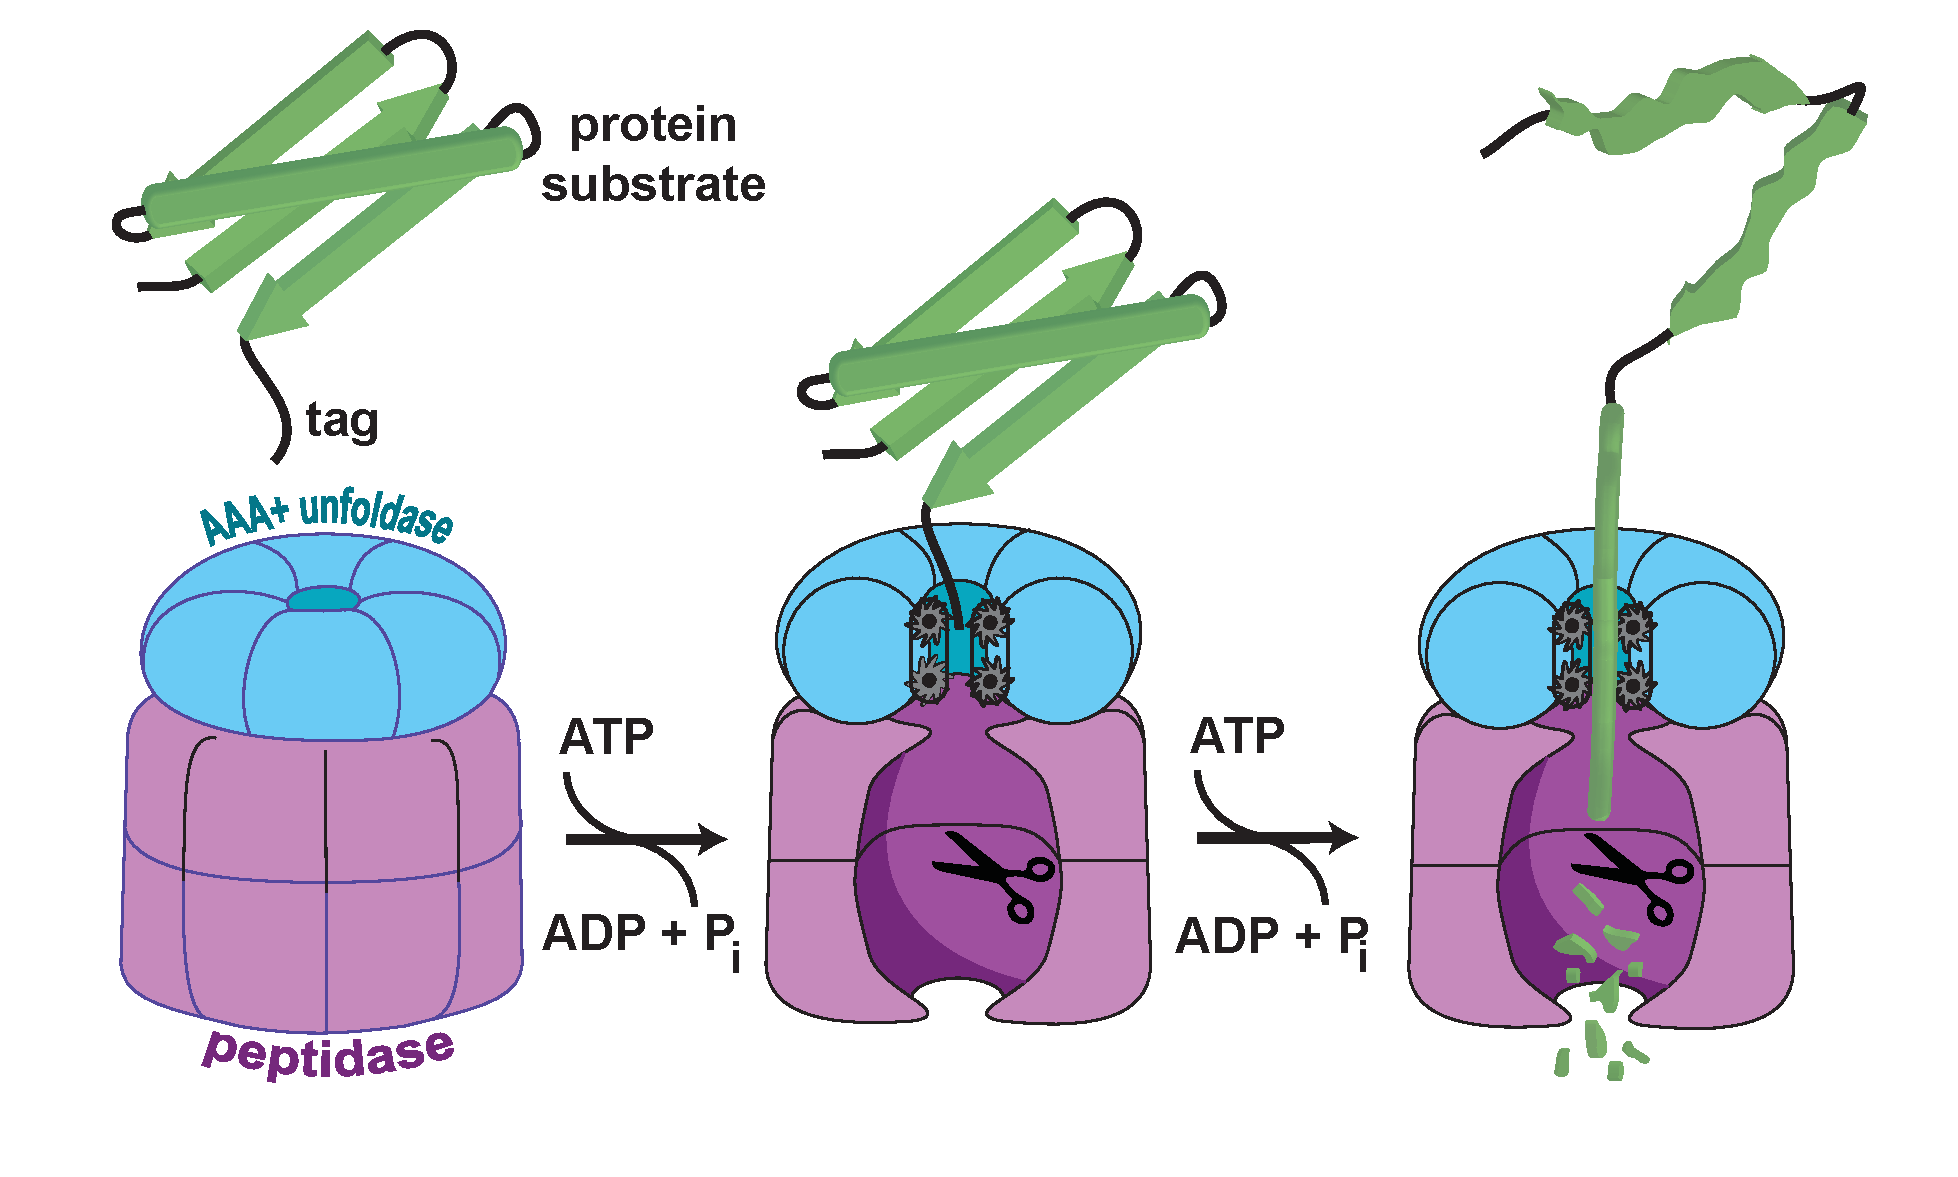
\includegraphics[scale=.4]{protease_robyn}% 
}
\caption[title]{title.\par
Adapted from ~\citet{Nyquist2014}. 
}
\label{fig:wbsto}
\end{figure}
%%-------------------------



CP active sites

large and small AAA+ domains, coordinated ATP hydrolysis

central pore, pore loops
power strokes
subunit communication
interface of unfoldase and peptidase



prokaryotic vs eukaryotic

\section{26S proteasome structure and assembly}
%EM 26S structure and subcomplexes
%base subunit architecture, EM structure and subunit schematic
%assembly

core
lid
base
chaperones
tails

complexity

\section{Steps in substrate processing}
%derivative of mary's schematic
ubiquitin binding
engagement
translocation and unfolding
deubiquitination - ubiqitin recycling
degradation - peptide release

ubiquitin chain linkage/length - affinity, binding orientation
substrate geometry - engagement
substrate stability - translocaton and unfolding 

how does heterohexameric architecture contribute to added complexity


\

\section{AAA+ protein unfoldases}
%active site
% top view with pore loops (pan or clpx?)
%rpt seq alignment (or put in main text as data?)

conserved AAA+ motifs
catalytic cycle
rigid body
pore loops
interaction with peptidase

\section{Subunit specialization in the heterohexameric AAA+ unfoldase of the proteasome}
	In this dissertation, we explore how the six distinct ATPase subunits of the proteasomal unfoldase are involved in substrate processing, interaction with the core peptidase and coordinated ATP hydrolysis.  To accomplish unprecedented systematic \textit{in vitro} studies, we developed a heterologous expression system to produce the unfoldase subcomplex from \textit{S. cerevisieae} in \textit{E. coli} and established conditions to reconstitute partially recombinant 26S proteasomes (Chapter~\ref{Chapter2}).\par
	Detailed analysis of the individual roles of the six proteasomal ATPase subunits in substrate processing required the biochemical characterization of catalytic mutations in conserved AAA+ motifs.  A mutation in the canonical AAA+ Walker\--B motif was used to trap single subunits in a defined ATP-bound state in order to define the contributions of individual subunits to substrate processing.  We demonstrate that the six ATPase subunits are functionally distinct and that ATP hydrolysis by Rpt3, Rpt4 and Rpt6 is crucial for successful substrate degradation.  These subunits are located at the top of the spiral staircase configuration of ATPases observed in the proteasomal unfoldase in absence of substrate, indicating that ATP hydrolysis may these subunits is potentially required for substrate engagement. (TRANSITION) We examined the importance of individual ATPase subunits for base-core association and demonstrated that peptidase binding and gate opening do not depend on the nucleotide state of specific Rpt C-terminal tails (Chapter~\ref{Chapter3}).\par
	Pursuant to these studies we explored the coordination of ATP hydrolysis within the base ATPase ring by  mutating the arginine finger to disrupt communication between neighboring subunits.  We further developed a series of concatamer substrates to deconvolute the processes of substrate engagement verses translocation by the proteasome base.  This tool will facilitate a more mechanistic understanding of how various mutants compromise substrate processing by the proteasome (Chapter~\ref{Chapter4}).\par
	Prior to these studies we lacked an understanding of how the heterohexameric architecture of the base unfoldase affects proteasomal substrate processing or subcomplex interactions.  Our work provides systematic and quantitative insights into the specialization of ATPase subunits in various aspects of proteasome function, including substrate engagement and translocation, interaction with the core peptidase, and the coordination of ATP hydrolysis.\par
	

